\section{Impact of cell errors on cross-point ReRAM Design}
\label{sec:intro}

Reliability is a vital concern in the design of memory system. In the cross-point structure, the reliability issues comes from two different sources: \emph{\textbf{structural error}} and \emph{\textbf{cell error}}. The structural error comes from the special organization of the cross-point array. The impact of voltage drop, sneak current, write/read schemes, as well as data pattern on the array reliability are well studied in literatures~\cite{jiale,Dimin_ISLPED}. It has been shown that the structural errors can be mitigated or eliminated with exhaustive worst-case design. On the other hand, because of the intrinsic characteristics of ReRAM cells, the impact of cell errors is not avoidable. To implement a reliable ReRAM array, additional detection and recovery mechanisms and circuity are required. In this section, we first discussed the resistance switching behaviors of ReRAM cell. Based on the discussion, mechanisms and modeling of soft error and hard error of ReRAM cell is presented. Then, the impact of the cell errors at the array design is evaluated.

\subsection{ReRAM resistance switching mechanisms}
%A schematic view of the switching mechanisms of ReRAM cell is illustrated in Fig. ~\ref{fig:filament}.
There are several studies have been conducted to reveal the physical mechanisms of the resistance switching behaviors. Recently, the filamentary model is widely accepted to explain the resistance switching phenomenon in the TMOs ReRAM: switchings between LRS and HRS are caused by the formation and rapture of the nanoscale conductive filaments (CFs) at the anode interface of the cell. For forming operation can be considered as a 'preset` operation of the ReRAM cell. The schematic view of the switching mechanisms of ReRAM cell is illustrated in Fig. ~\ref{fig:filament}.

During the forming step, a high voltage is applied across the cell. The dielectric soft breakdown in the materials generates a great amount of the defects in the TMOs, which form one or several CFs through the cell. At the same time, the anode becomes a reservoir of the oxygen ions. After the forming operation, the cell exhibit LRS, which is shown in Fig.~\ref{fig:filament}(a). The RESET operation is shown in Fig.~\ref{fig:filament}(b). In this step, the oxygen ions are forced back to the TMO layer by the electric field and recombine with the oxygen vacancies (Vo). In this case, the CFs are ``cut doff'' and the cell becomes HRS, which is shown in Fig.~\ref{fig:filament}(d). In contrast, the SET operation can be considered as a converse process of the RESET operation. As shown in Fig.~\ref{fig:filament}(c), the SET operation realizes the regeneration of the CFs by separating the oxygen ions and the Vo again. In this case, the cell switches back to the LRS.
\begin{figure}[!t]
\centering
    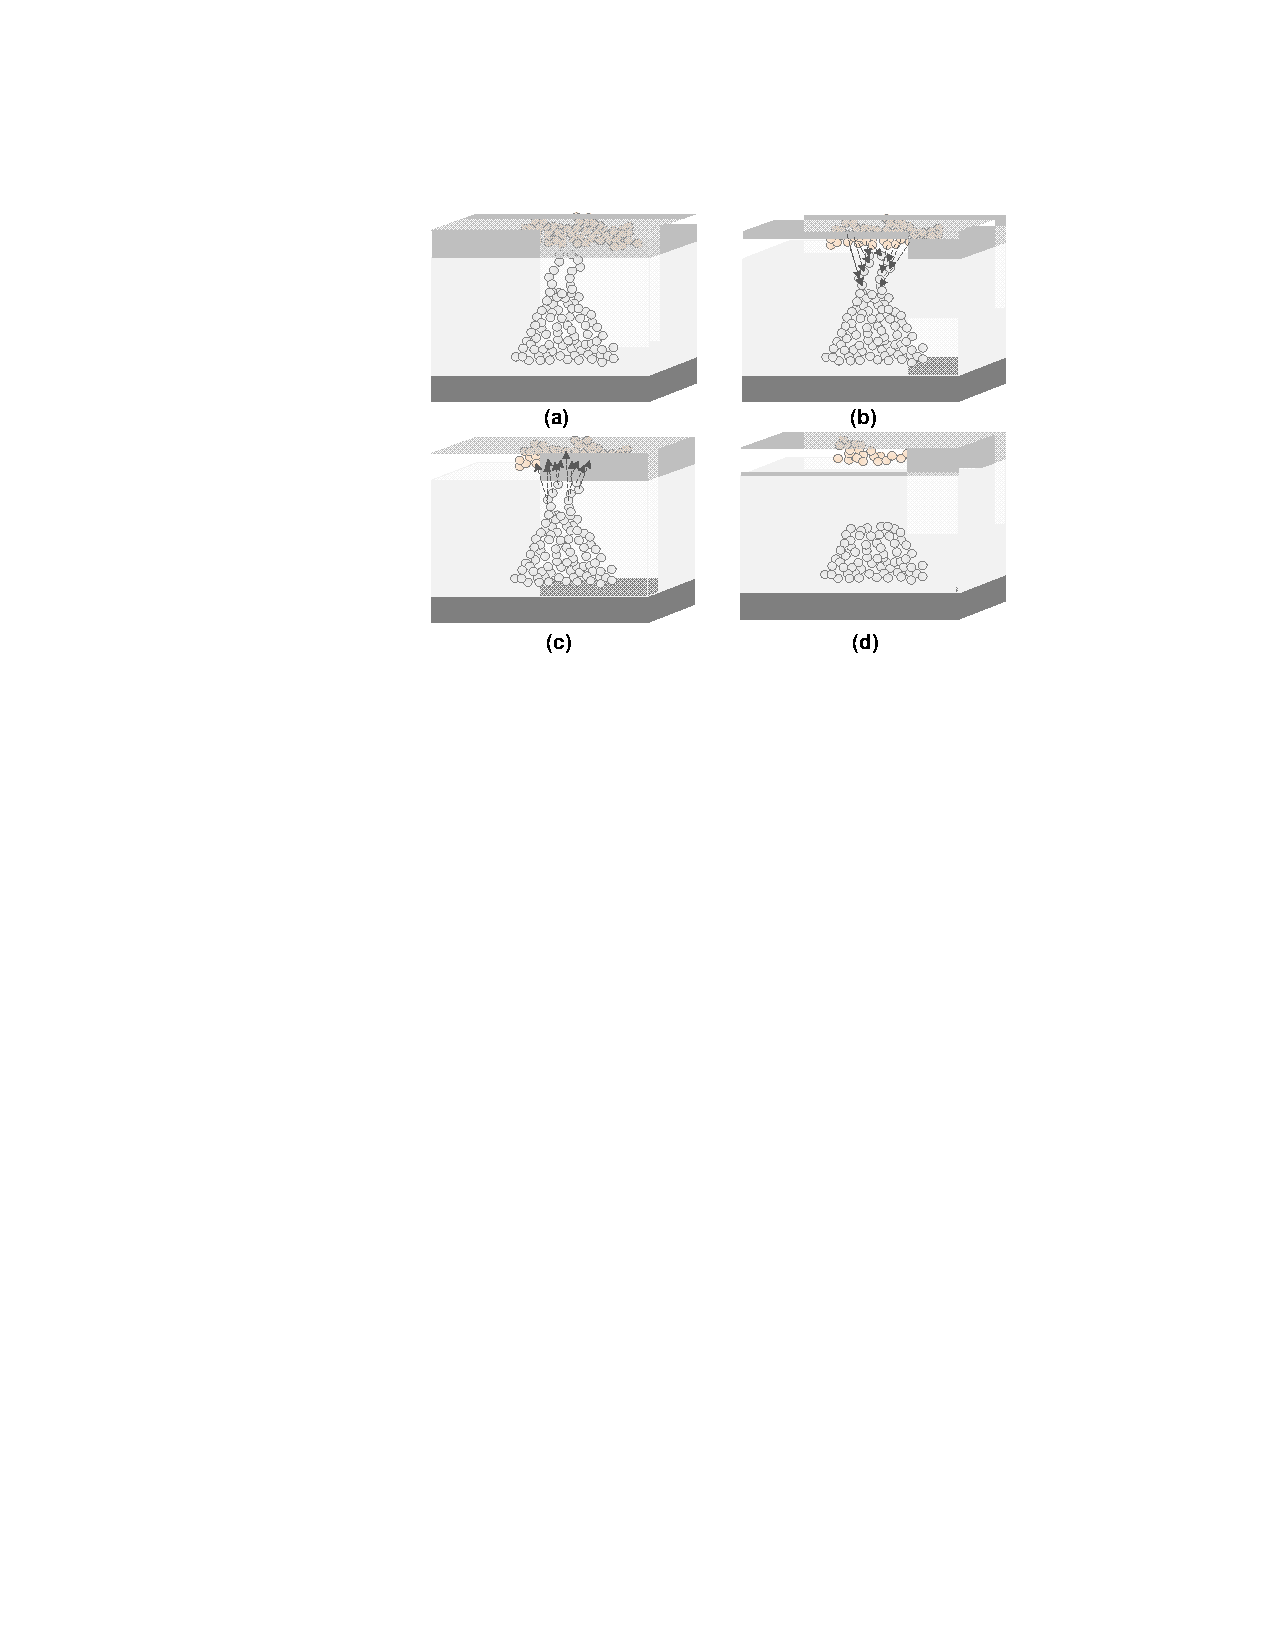
\includegraphics[width=3.5in]{./fig/DATE2.pdf}
\caption{(a) LRS of the ReRAM cell after the formation or SET operation.  (b) RESET operation. (c) HRS of the ReRAM cell after RESET operation. (4) SET operation.}
\label{fig:filament}
\end{figure}

\subsection{Mechanisms and Modeling of Soft Error and Hard Error of ReRAM} \label{sec:Model}

Soft error of the ReRAM cell come from the retention error. The retention failure is a recoverable upset of the resistance of the cell. The retention failure can either be a suddenly resistance drop of the HRS cell (HRS failure) or a suddenly resistance increasing of the LRS cell (LRS failure). The retention failure behaviors result from the random generation of the Vo (HRS failure), and the recombination of Vo with oxygen ions (LRS failure). Both of them imply that the retention failure is a random phenomenon rather than a cumulative phenomenon. Since either of the HRS failure or the LRS failure can be the dominate soft error of the ReRAM with different materials and process technology~\cite{softerror_yu,softerror_gao}, in this paper, we focus on the soft error that dominated by the LRS failure.

In order to quantify the retention failure behavior,the cumulative failure probability is employed. A simplified model of the cumulative failure probability is proposed by Gao~\cite{softerror_gao}, which can be expressed as
\begin{equation}
F(t) = 1-(1-p)^{(\alpha t)},
\end{equation}
where $\alpha$ is a constant value, $t$ is the retention time, ad $p$ is the generation probability of the Vo and has the term of
\begin{equation}
p_H = exp((qVl/2d-\varepsilon_V)/kT),
\end{equation}
where $q$ is the electric quantity if the oxygen ions, $V$ is the applied voltage on the TMO layer, $l$ is the lattice constant, $d$ is the length of the filament's ruptured region, and the $\varepsilon_V$ is the oxygen vacancy's formation energy.

Different from soft error, the hard error results from the limited endurance of the ReRAM cell compared to traditional DRAM/SRAM technologies. The endurance failure is caused by a gradually resistance change over the write cycles. According to different behaviors and physical mechanisms, the endurance failures are classified into three categories~\cite{harderror}:
\begin{enumerate}
  \item Type I Failure: This failure is caused by the generation of extra oxide layer at the anode during the SET operations. This layer prevents the moving of the oxygen ions and results in the increased $R_{LRS}$ and the degreased $R_{HRS}$.
  \item Type II Failure: The programming voltage generated extra Vo, which directly increases the diameter of the CFs. In this failure, both of the $R_{LRS}$ and the $R_{HRS}$ decreases gradually.
  \item Type III Failure:This failure results from the undesired consumption of the oxygen ions at stored in the anode. In this case, the combination probability of Vo and oxygen ions will reduce. Thus the $R_{HRS}$ decreases while the $R_{LRS}$ keeps constant.
\end{enumerate}

\begin{figure}[!t]
\centering
    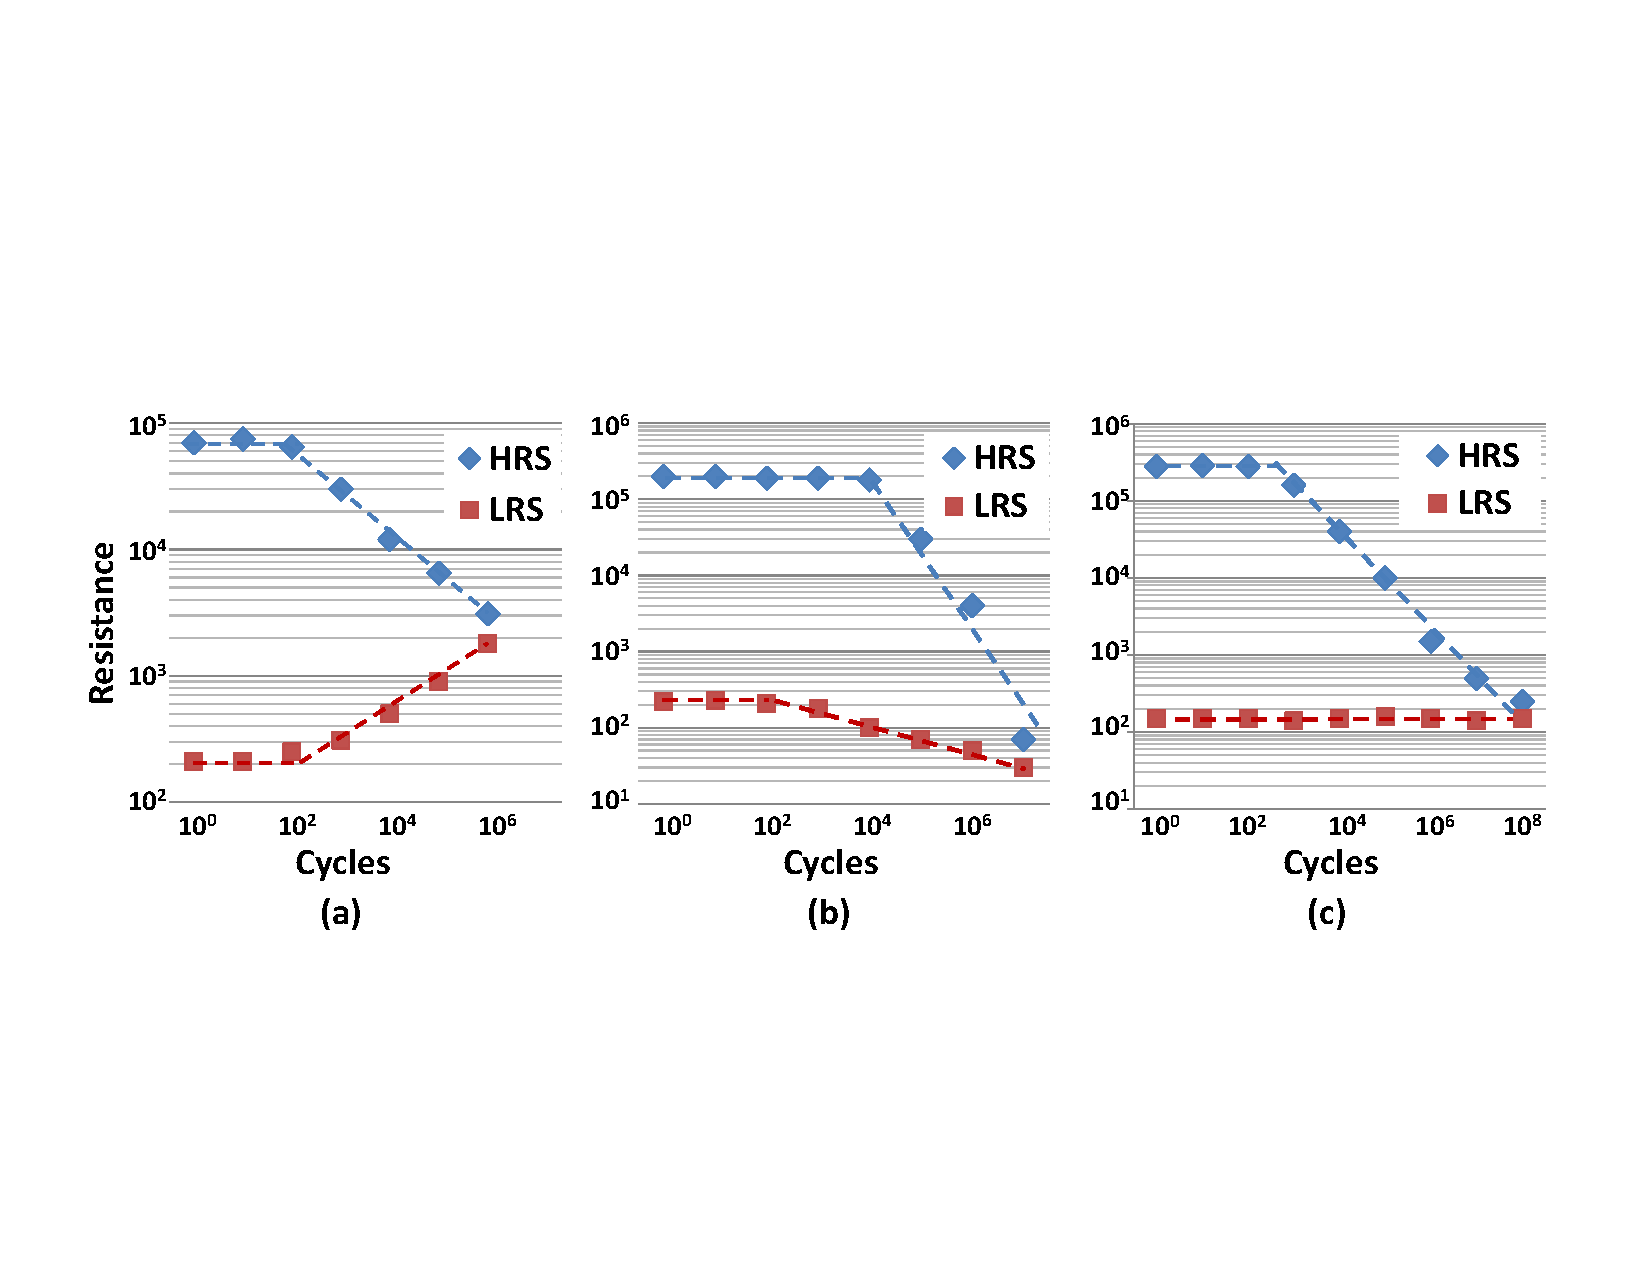
\includegraphics[width=3.5in]{./fig/errors.pdf}
\caption{Hard errors in TMO ReRAM cell: (a) Type I, (b) Type II, and (c) Type III endurance failure.}
\label{fig:errors}
\end{figure}
For simplicity, we proposed a unified model to summarize these three types of endurance failure as
\begin{equation}
R = R_0(1+{\alpha_0(t-t_0)^{\xi}(sgn(t-t_0)+1)/2}),
\end{equation}
where $R_0$ is the initial resistance of LRS or HRS, $t_0$ is the start point that the endurance degradation is observed, and $\alpha_0$ and ${\xi}$ represent the direction and speed of the resistance change. The model with different parameters fits good with the published data and is shown in Fig.~\ref{fig:errors} as dash lines.

\subsection{Impact of Soft and Hard Error on Cross-point Array}
%    512 x 512
%    R_line = 0.65
%    R_h = 500 000;
%    R_l =  20 000;  R_l_half = 100 000;
%    Kr = 10;
%    R_read = 100 000;
%    R_read_h =1 000 000;
The soft error is a recoverable error and represents as a HRS-to-LRS or LRS-to-HRS transition. Therefore, we conclude that soft errors can only affect the information stored in the cells where the endurance failures arise, and will not affect the other cells in the cross-point array. To overcome the soft error, the Error Correction Code (ECC) is necessary. The area, energy, and latency overheads will be evaluate in Section~\ref{sec:expe}.

Compared to the soft errors, the hard errors are more serious, especially for the cross-point structure. In general, the impact of hard errors exists in two aspects: (1) the degradation of the read margin results from the shrink of the resistance ration between the HRS and the LRS. This problem appears in all of three types hard errors; (2) the design overhead that incurred by the hard errors, including the area overhead, energy consumption overhear, as well as more severe array size limitation. However, since the LRS is the decisive for the worst-case design, only the Type II hear error will affect the design.


Fig.~\ref{fig:margin} shows the read margin degradation results from the resistance change of the HRS and LRS. According to the aforementioned Type I-III hard errors, the endurance failures of HRS always represent the resistance reduction. However, the resistance of LRS may either increases (for Type I error) or decreases (for Type II error). Therefore, in this figure, we assume the resistance of HRS can reduce to half of the original value, while that of LRS can either increase or decrease by 50\% of the original value. From the figure, we can see that the reduction of the resistance ratio between HRS and LRS, which results from the resistance increasing of LRS and decreasing of HRS, has significant impact on the read margin. For example, when the resistance of LRS reduces by 50\%, the read margin will reduce by 35\%. And when the resistance of HRS increase by 50\%, the read margin shrinks to only 1.2\% of the original read margin. This observation indicates that the HRS endurance failure brings more serious degradation to the read noise margin. 

%In addition, our simulation also shows that the endurance failures can also make the array unreadable for specific HRS resistance increasing and LRS resistance decreasing. In our simulation, XXXXXXXXXXX Inditace the unreadable region.

\begin{figure}[!t]
\centering
    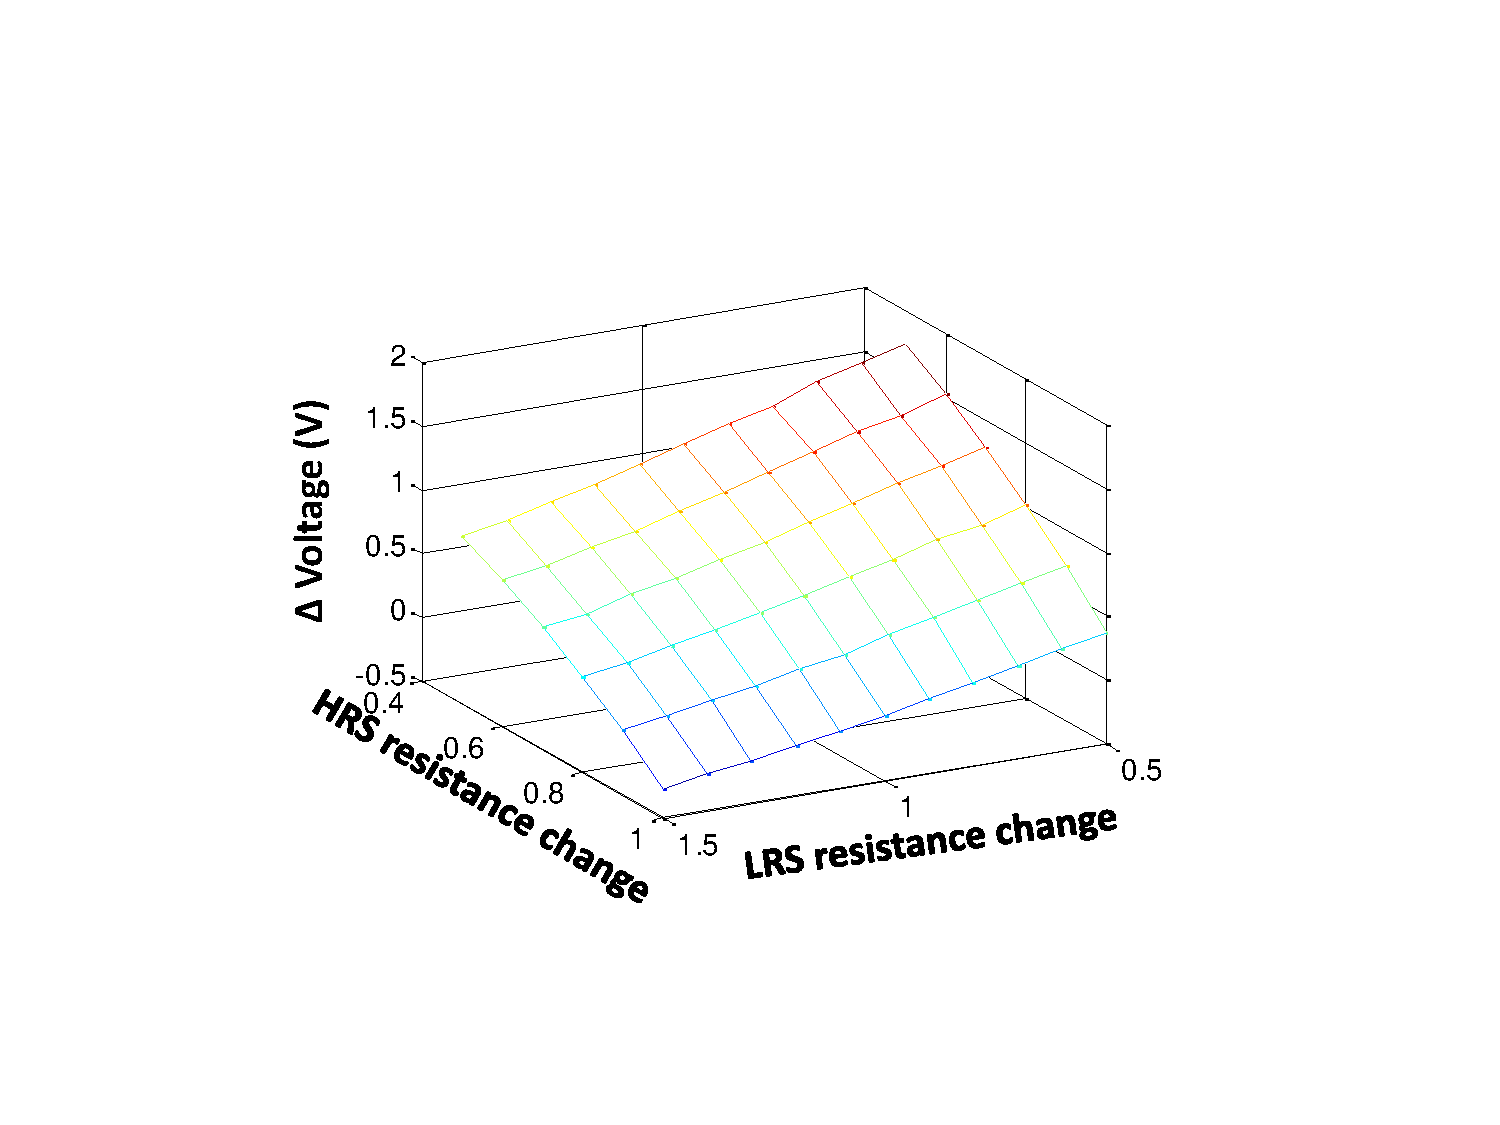
\includegraphics[width=2in]{./fig/margin.pdf}
\caption{Impact of endurance failures on read margin.}
\label{fig:margin}
\end{figure}


As mentioned, to overcome the hard errors, the design limitations of the cross-point array is further deteriorated. To ensure the reliability of the array, the cross-point array is always designed for the worst case - making sure that the array can work reliably, regardless the data pattern in the array. Many researches have been conducted to study the worst case design~\cite{jiale, Dimin_ISLPED} and it has been figure out that the lowest resistance is the key parameter for the worst case design of cross-point array. Since the LRS resistance reduction is only observed in Type II error, therefore, we conclude the Type II hard error is the key player for the worst case design. Firstly, the limitation of the array size results from the voltage drop along the wordlines and bitlines. Our simulation shows that the decrease of the resistance of LRS will aggravate the voltage drop and therefor reduce the allowable array size. As shown in Fig.~\ref{fig:size}, the maximum array size reduces from 512 by 512 to 355 by 355 with the LRS resistance drop to half of its original value. Besides, the energy consumption and the driver current are also impact by the LRS resistance reduction. Fig.~\ref{fig:EC} shows the energy and driver current overhead of the LRS resistance reduction. As shown, the worst case energy consumption of the array increases by 55\%. On the other hand, the driver current in increases up to 72\%. Since the area of the wordline voltage driver and bitline multiplexors is linearly related to the driver current requirement, the area of peripheral circuits are also harmed.


%As mentioned, the existence of the voltage drops along the metal wires and the sneak paths brings in extra reliability issues to the cross-point array design. Firstly, the maximum array size will be reduced due to the hard error. In cross-point array, the

\begin{figure}[!t]
\centering
    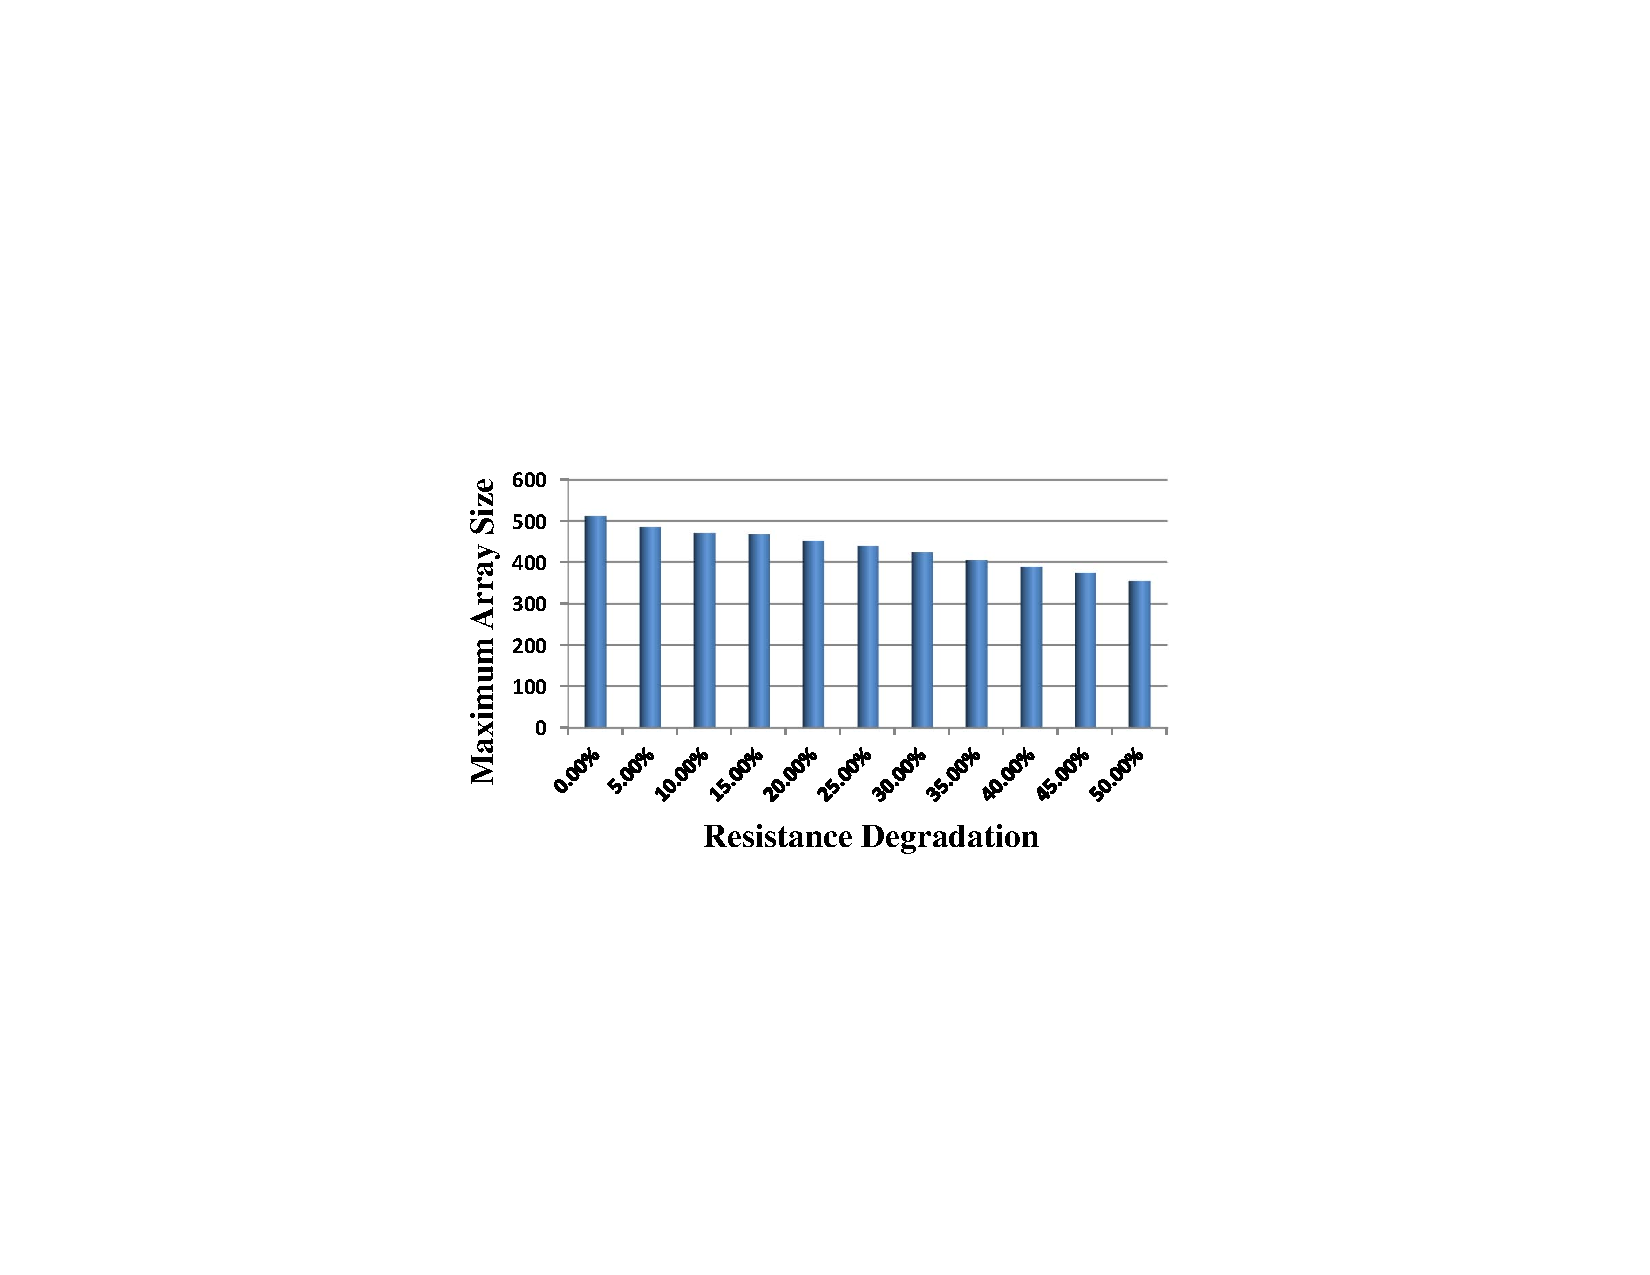
\includegraphics[width=2.5in]{./fig/size.pdf}
\caption{Impact of Type II error on maximum array size.}
\label{fig:size}
\end{figure}

\begin{figure}[!t]
\centering
    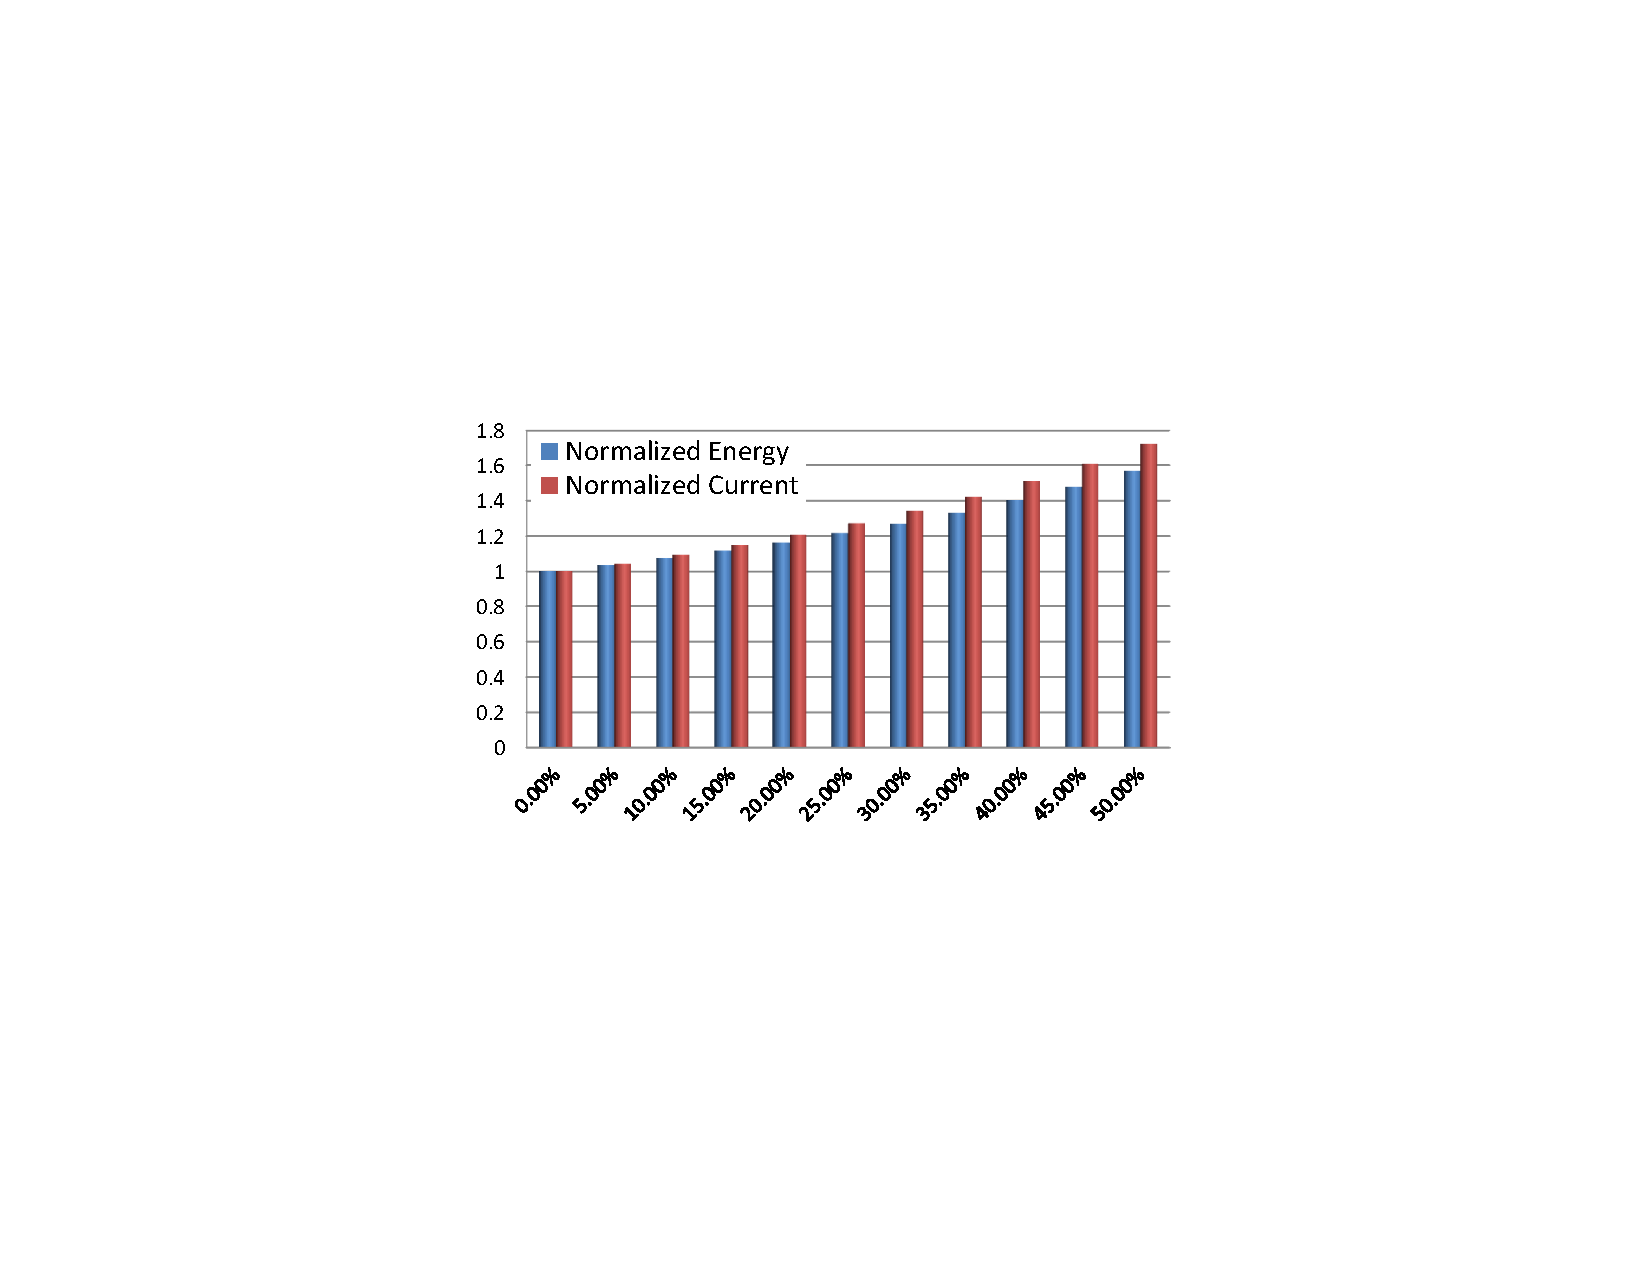
\includegraphics[width=2.5in]{./fig/EC.pdf}
\caption{Impact of Type II error on energy consumption and current requirement.}
\label{fig:EC}
\end{figure}
